%COMANDO CHE DETERMINA IL TIPO DI DOCUMENTO CHE SI VUOLE CREARE

\documentclass[a4paper,12pt]{report}

%ELENCO DEI PACCHETTI UTILI PER LA STESURA DEL DOCUMENTO

\usepackage[utf8]{inputenc}
\usepackage[english, italian]{babel}
\usepackage{graphicx}
\usepackage{float}
\usepackage{tabularx}
\usepackage{makecell}
\usepackage{titlesec}
\usepackage{fancyhdr}
\usepackage{lastpage}
\usepackage{xurl}
\usepackage{hyperref}
\usepackage{geometry}
\usepackage[table,dvipsnames]{xcolor}
\setcounter{tocdepth}{5}
\setcounter{secnumdepth}{5}
\usepackage{caption}
\usepackage{etoolbox}% >= v2.1 2011-01-03
\usepackage{tikz}
\usepackage{listings}
\usepackage{scalerel}
\usepackage{longtable}
\usepackage{comment}
\usepackage{amssymb}
\usepackage{listings}

\titleformat{\chapter}[display]
{\normalfont\bfseries}{}{0pt}{\LARGE}

%COMANDO PER LA SPAZIATURA DEI TITOLI DAL BORDO DEL FOGLIO

\titlespacing*{\chapter}{0cm}{0cm}{0.2cm}

%COMANDO PER LA SPAZIATURA DEL TESTO DAI BORDI LATERALI

\geometry{
	left=20mm,
	right=20mm,
}

%COMADNO PER AVERE L'INDICE DEL NOME CHE SI VUOLE

\renewcommand{\contentsname}{Indice}

%COMADNI PER OTTENERE SUBSUBSECTION NUMERATE E PRESENTI NELL'INDICE

\setcounter{tocdepth}{5}
\setcounter{secnumdepth}{5}

%COMANDI PER OTTENERE HEADER E FOOTER

\pagestyle{plain}

\fancypagestyle{plain}{
	\fancyhf{}
	\lhead{
\includegraphics[width=3cm]{../../immagini/minilogo.jpg}}
	\chead{}
	\rhead{\fontsize{12}{10}Verbale Esterno 2021-04-15}
	\lfoot{}
	\cfoot{\thepage\ di \pageref{LastPage}}
	\rfoot{}
}

\pagestyle{plain}

%COMANDI PER LINK

\hypersetup{
	colorlinks=true,
	linkcolor=black,
	filecolor=black,
	urlcolor=blue,
	citecolor=black,
}

%COMANDI PER SNIPPET DI CODICE

\BeforeBeginEnvironment{lstlisting}{\begin{mdframed}\vspace{-0.7em}}
	\AfterEndEnvironment{lstlisting}{\vspace{-0.5em}\end{mdframed}}

% needed for \lstcapt
\def\ifempty#1{\def\temparg{#1}\ifx\temparg\empty}

% make new caption command for listings
\usepackage{caption}
\newcommand{\lstcapt}[2][]{%
	\ifempty{#1}%
	\captionof{lstlisting}{#2}%
	\else%
	\captionof{lstlisting}[#1]{#2}%
	\fi%
	\vspace{0.75\baselineskip}%
}

\definecolor{atomlightorange}{rgb}{0.88,0.76,0.55}
\definecolor{atomdarkgrey}{RGB}{59,62,75}

% set listings
\lstset{%
	basicstyle=\footnotesize\ttfamily\color{atomlightorange},
	framesep=20pt,
	belowskip=10pt,
	aboveskip=10pt
}

% add frame environment
\usepackage[%
framemethod=tikz,
skipbelow=8pt,
skipabove=13pt
]{mdframed}
\mdfsetup{%
	leftmargin=0pt,
	rightmargin=0pt,
	backgroundcolor=atomdarkgrey,
	middlelinecolor=atomdarkgrey,
	roundcorner=6
}

%BIBLIOGRAFIA

\makeatletter
\def\thebibliography#1{\chapter*{Bibliografia\@mkboth
		{Bibliografia}{Bibliografia}}\list
	{[\arabic{enumi}]}{\settowidth\labelwidth{[#1]}\leftmargin\labelwidth
		\advance\leftmargin\labelsep
		\usecounter{enumi}}
	\def\newblock{\hskip .11em plus .33em minus .07em}
	\sloppy\clubpenalty4000\widowpenalty4000
	\sfcode`\.=1000\relax}
\makeatother

%DEFINIZIONE COLORI

\definecolor{airforceblue}{rgb}{0.36, 0.54, 0.66}


\begin{document}
\makeatletter
\begin{titlepage}
	\begin{center}
		\vspace*{-4cm}
		\author{Jawa Druids}
		\title{Manuale Sviluppatore}
		\date{} %LASCIARE QUESTO CAMPO VUOTO, SE LO TOLGO STAMPA LA DATA CORRENTE
		
\includegraphics[width=0.5\linewidth]{../immagini/DRUIDSLOGO.jpg}\\[4ex]
		{\huge \bfseries  \@title }\\[2ex]
		{\LARGE  \@author}\\[50ex]
		\vspace*{-9cm}
		\begin{table}[H]
			\renewcommand{\arraystretch}{1.4}
			\centering
			\begin{tabular}{r | l}
				\textbf{Versione} & 1.0.0 \\%RIGA PER INSERIRE LA VERSIONE ULTIMA DEL DOCUMENTO
				\textbf{Data approvazione} & 2021-04-26 \\
				\textbf{Responsabile} & Mattia Cocco \\
				\textbf{Redattori} & \makecell[tl]{Mattia Cocco \\ Andrea Dorigo \\ Alfredo Graziano} \\
				\textbf{Verificatori} & \makecell[tl]{Andrea Cecchin} \\
				%MAKECELL SERVE PER POI ANDARE A CAPO ALL'INTERNO DELLA CELLA
				\textbf{Stato} & Approvato\\
				\textbf{Lista distribuzione} & \makecell[tl]{Jawa Druids \\ Prof. Tullio Vardanega \\ Prof. Riccardo Cardin}\\
				\textbf{Uso} & Esterno
			\end{tabular}
		\end{table}
		\vspace{0.1cm}
		\hfill \break
		\fontsize{17}{10}\textbf{Sommario} \\
		\vspace{0.1cm}
		Il documento ha lo scopo di presentare le tecnologie e l'architettura del sistema agli sviluppatori interessati al software \emph{\normalsize{\textit{GDP - Gathering Detection Platform}}}.
	\end{center}
\end{titlepage}
\makeatother
	\quad
\begin{center}
	\LARGE\textbf{Registro delle modifiche}
\end{center}
\def\tabularxcolumn#1{m{#1}}
{\rowcolors{2}{RawSienna!90!RawSienna!20}{RawSienna!70!RawSienna!40}

\begin{center}
	\renewcommand{\arraystretch}{1.4}
	\begin{longtable}{|p{4cm}|p{3cm}|p{2.8cm}|p{2cm}|p{1.7cm}|}
	\hline
	\rowcolor{airforceblue}
	\textbf{Modifica} & \textbf{Autore} & \textbf{Ruolo} & \textbf{Data} & \textbf{Versione}
	\\
	\hline
	\textit{Approvazione del documento per RR} & Igli Mezini & \textit{Responsabile} & 10-01-2021 & v1.0.0
	\\
	\hline
	\textit{Revisione Finale del documento} & Margherita Mitillo & \textit{Verificatore} & 09-01-2021 & v0.9.0
	\\
	\hline
	\textit{Verificato capitolo \S~\ref{Formazione}} & Margherita Mitillo & \textit{Verificatore} & 08-01-2021 & v0.8.0
	\\
	\hline
	\textit{Verificate sezioni \S~\ref{ProcessiPrimariProgettazione}, \S~\ref{ProcessiPrimariCodifica}, \S~\ref{ProcessiPrimariStrumenti}, \S~\ref{Standard ISO/IEC 15504} } & Andrea Dorigo & \textit{Verificatore} & 08-01-2021 & v0.7.0
	\\
	\hline
	\textit{Verificate sezioni \S~\ref{ProcessiDiSupportoGestioneDellaConfigurazione}, \S~\ref{ProcessiOrganizzativiProcessoDiPianificazione}, \S~\ref{ProcessiOrganizzativiFormazione}} & Margherita Mitillo & \textit{Verificatore} & 07-01-2021 & v0.6.0
	\\
	\hline
	\textit{Verificate sezioni \S~\ref{ProcessiDiSupportoVerifica}, \S~\ref{ProcessiDiSupportoValidazione}, \S~\ref{StandardISO/IEC9126}} & Emma Roveroni & \textit{Verificatore} & 07-01-2021 & v0.5.0
	\\
	\hline
	\textit{Aggiunto capitolo \S~\ref{Formazione}} & Mattia Cocco & \textit{Amministratore} & 06-01-2021 & v0.4.7
	\\
	\hline
	\textit{Aggiunte sezioni \S~\ref{ProcessiDiSupportoVerifica} e \S~\ref{ProcessiDiSupportoValidazione} } & Alfredo Graziano & \textit{Amministratore} & 05-01-2021 & v0.4.6
	\\
	\hline
	\textit{Aggiunto capitolo \S~\ref{ProcessiOrganizzativiFormazione}} & Mattia Cocco & \textit{Amministratore} & 05-01-2021 & v0.4.5
	\\
	\hline
	\textit{Aggiunte sezioni \S~\ref{ProcessiPrimariProgettazione}, \S~\ref{ProcessiPrimariCodifica}, \S~\ref{ProcessiPrimariStrumenti}} & Andrea Cecchin & \textit{Amministratore} & 03-01-2021 & v0.4.4
	\\
	\hline
	\textit{Aggiunta sezione \S~\ref{ProcessiDiSupportoGestioneDellaConfigurazione}} & Andrea Dorigo & \textit{Amministratore} & 02-01-2021 & v0.4.3
	\\
	\hline
	\textit{Aggiunte sezioni \S~\ref{ProcessiPrimariProspettiveAnalisiDeiRequisitiMetriche}, \S~\ref{ProcessiDiSupportoVerificaDescrizione}} & Mattia Cocco & \textit{Amministratore} & 02-01-2021 & v0.4.2
	\\
	\hline
	\textit{Aggiunto capitolo \S~\ref{Standard ISO/IEC 15504}} & Alfredo Graziano & \textit{Amministratore} & 01-01-2021 & v0.4.1
	\\
	\hline
	\textit{Verificate sezioni \S~\ref{ProcessiDiSupportoGestioneDellaQualità} e \S~\ref{ProcessiOrganizzativiProcessoDiCoordinamento} } & Emma Roveroni & \textit{Verificatore} & 31-12-2020 & v0.4.0
	\\
	\hline
	\textit{Aggiunta sezione \S~\ref{ProcessiOrganizzativiProcessoDiPianificazioneMetriche}} & Alfredo Graziano & \textit{Amministratore} & 30-12-2020 & v0.3.4
	\\
	\hline
	\textit{Aggiunte sezioni \S~\ref{ProcessiDiSupportoGestioneDellaQualità}, \S~\ref{StandardISO/IEC9126} } & Mattia Cocco & \textit{Amministratore} & 30-12-2020 & v0.3.3
	\\
	\hline
	\textit{Aggiunte sezioni \S~\ref{ProcessiOrganizzativiProcessoDiPianificazioneScopo}, \S~\ref{ProcessiOrganizzativiProcessoDiPianificazioneRuoliDiProgetto}, \S~\ref{ProcessiOrganizzativiProcessoDiPianificazioneAssegnazioneDeiCompiti}, \S~\ref{ProcessiOrganizzativiProcessoDiPianificazioneTrelloEGitkraken}, \S~\ref{ProcessiOrganizzativiProcessoDiPianificazioneStrumenti} } & Igli Mezini & \textit{Amministratore} & 30-12-2020 & v0.3.2
	\\
	\hline
	\textit{Aggiunte sezioni \S~\ref{ProcessiOrganizzativiProcessoDiCoordinamentoScopo}, \S~\ref{ProcessiOrganizzativiProcessoDiCoordinamentoComunicazione}, \S~\ref{ProcessiOrganizzativiProcessoDiCoordinamentoRiunioni}, \S~\ref{ProcessiOrganizzativiProcessoDiCoordinamentoStrumentiUtilizzatiPerIlProcessoDiCoordinamento} } & Igli Mezini & \textit{Amministratore} & 29-12-2020 & v0.3.1
	\\
	\hline
	\textit{Verificata sezione \S~\ref{ProcessiDiSupportoDocumentazione}} & Andrea Dorigo & \textit{Verificatore} & 15-12-2020 & v0.3.0
	\\
	\hline
	\textit{Verificate sezioni \S~\ref{ProcessiPrimariFornitura} e \S~\ref{ProcessiPrimariSviluppo} } & Margherita Mitillo & \textit{Verificatore} & 11-12-2020 & v0.2.0
	\\
	\hline
	\textit{Verificato capitolo \S~\ref{Introduzione}} & Margherita Mitillo & \textit{Verificatore} & 10-12-2020 & v0.1.0
	\\
	\hline
	\textit{Aggiunte sezioni \S~\ref{ProcessiDiSupportoDocumentazioneMetricheCorrettezzaOrtografica}, \S~\ref{ProcessiDiSupportoDocumentazioneDirectoryDiUnDocumento}} & Andrea Dorigo & \textit{Amministratore} & 08-12-2020 & v0.0.9
	\\
	\hline
	\textit{Aggiunte sezioni \S~\ref{ProcessiDiSupportoDocumentazioneMetriche}, \S~\ref{ProcessiDiSupportoDocumentazioneStrumentiDiStesura}} & Igli Mezini & \textit{Amministratore} & 03-12-2020 & v0.0.8
	\\
	\hline
	\textit{Aggiunte sezioni \S~\ref{ProcessiDiSupportoDocumentazioneStrutturaGeneraleDeiDocumenti}, \S~\ref{ProcessiDiSupportoDocumentazioneNormeTipografiche}, \S~\ref{ProcessiDiSupportoDocumentazioneElementiGrafici}} & Igli Mezini & \textit{Amministratore} & 01-12-2020 & v0.0.7
	\\
	\hline
	\textit{Aggiunta sezione \S~\ref{ProcessiPrimariSviluppo}} & Andrea Cecchin & \textit{Amministratore} & 30-11-2020 & v0.0.6
	\\
	\hline
	\textit{Aggiunte sezioni \S~\ref{ProcessiDiSupportoDocumentazioneTemplateInFormatoLatex}, \S~\ref{ProcessiDiSupportoDocumentazioneDocumentiProdotti}, \S~\ref{ProcessiDiSupportoDocumentazioneDirectoryDiUnDocumento}} & Igli Mezini & \textit{Amministratore} & 29-11-2020 & v0.0.5
	\\
	\hline
	\textit{Aggiunte sezioni \S~\ref{ProcessiDiSupportoDocumentazioneDescrizione}, \S~\ref{ProcessiDiSupportoDocumentazioneImplementazioneDelDocumento}, \S~\ref{ProcessiDiSupportoDocumentazioneCicloDiVitaDiUnDocumento}} & Igli Mezini & \textit{Amministratore} & 28-11-2020 & v0.0.4
	\\
	\hline
	\textit{Aggiunte sezioni \S~\ref{ProcessiPrimariFornituraStudioDiFattibilità}, \S~\ref{ProcessiPrimariFornituraAltraDocumentazioneDaFornire}, \S~\ref{ProcessiPrimariFornituraStrumenti}} & Andrea Cecchin & \textit{Amministratore} & 26-11-2020 & v0.0.3
	\\
	\hline
	\textit{Aggiunte sezioni \S~\ref{Introduzione} e \S~\ref{ProcessiPrimariFornituraScopo}} & Andrea Cecchin & \textit{Amministratore} & 25-11-2020 & v0.0.2
	\\
	\hline
	\textit{Prima stesura del documento} & Andrea Cecchin & \textit{Amministratore} & 24-11-2020 & v0.0.1
	\\
	\hline
	\end{longtable}
\end{center}


	\tableofcontents{}
	\listoffigures{}
	\chapter{Introduzione}\label{Introduzione}

\section{Scopo del documento}
Il Piano di Qualifica è un documento su cui si prevede di operare per l’intera durata del progetto 
e il cui scopo è presentare e descrivere le strategie di verifica e validazione adottate 
dal gruppo Jawa Druids al fine di garantire la qualità di prodotto e di processo.  
Per raggiungere questo obbiettivo viene applicato un sistema di verifica continua sui processi in corso e 
sulle attività svolte, in modo da rilevare e correggere subito eventuali anomalie, riducendo lo spreco di risorse 
ed il rischio di reiterare gli stessi errori.
\section{Scopo del prodotto}
L'obiettivo del prodotto \textit{GDP - Gathering Detection Platform} di \textit{Sync Lab} è la creazione di un sistema software in 
grado di acquisire, monitorare, utilizzare e correlare tra loro tutti i dati acquisiti tramite sensoristica (come telecamere di videosorveglianza)
e altre sorgenti dati (es. orari con il maggior numero di visite degli esercizi commerciali estrapolati da Google) con lo
scopo di avere indicazioni di potenziali assembramenti e quindi di fornire supporto per trovare soluzioni che limitino tali condizioni.
\section{Glossario}
Al fine di favorire la comprensione totale della documentazione relativa al progetto, viene fornito un documento denominato \textit{Glossario -- fornire versione}
che riporta la spiegazione della terminologia specifica e tecnica utilizzata per la stesura di questo ed altri documenti.
Tali termini, quando utilizzati, vengono contrassegnati con un apice \textsuperscript{G} alla fine della parola.
\section{Standard di progetto}
Decidere se scrivere di aver utilizzato un determinato standard ISO per il software, se si, definirlo nelle norme di progetto!
\section{Riferimenti}
\subsection{Riferimenti normativi}
\begin{itemize}
	\item \textit{Norme di Progetto}
\end{itemize}
\subsection{Riferimenti informativi}
\begin{itemize}
	\item \textit{IEEE Recommended Practice for Software Requirements Specifications:}\\
	\url{https://ieeexplore.ieee.org/document/720574}
	\item \textit{Seminario per approfondimenti tecnici del capitolato C3:}\\
	\url{https://www.math.unipd.it/~tullio/IS-1/2020/Progetto/ST1.pdf}		
\end{itemize}
	\chapter{Requisiti di sistema}\label{RequisitiDiSistema}
\section{Requisiti minimi}\label{RequisitiDiSistemaRequisitiMinimi}
Il software è stato testato, con esito positivo, su di una macchina virtuale con i seguenti requisiti:
\begin{itemize}
  \item RAM: 4Gb;
  \item Solid State Drive: 10Gb;
  \item processore: Intel(R) Core(TM) i7-4710HQ CPU @ 2.50GHz CPU.
  \item Ubuntu 20.04 LTS
\end{itemize}
e su di un MacBook Air (early 2015) con le seguenti caratteristiche:
\begin{itemize}
  \item RAM: 4Gb;
  \item Solid State Drive: 128Gb;
  \item processore: Intel(R) Core(TM) i5 Dual Core @ 1.6GHz CPU.
  \item Mac OS v11.2.3
\end{itemize}

Nonostante non sia stato possibile fornire i requisiti minimi esatti a causa di mancanza di macchine fisiche, possiamo garantire che il software funzioni correttamente su macchine di specifiche simili o migliori.

\section{Browser}\label{RequisitiDiSistemaBrowser}
I browser sui quali è stato testato il software sono i seguenti:
\begin{itemize}
  \item Google Chrome v88 o superiore;
  \item Firefox developer v89.0b1 o superiore;
  \item Edge v87 superiore;
  \item Safari 14.0.3 o superiore.
\end{itemize}

	\chapter{Procedure di installazione}\label{ProceduraDiInstallazione}
Questa sezione esporrà le procedure di installazione all'interno del sistema operativo Linux$_G$, più precisamente Ubuntu$_G$ 20.04 LTS, in quanto utilizzato anche per lo sviluppo del software stesso.
Rimane comunque possibile installare il software su altri sistemi operativi soddisfando le dipendenze necessarie, ma non verrà qui esplicitato.

\section{Download della repository}\label{ProceduraDiInstallazioneDownloadRepo}
Per scaricare correttamente i contenuti della repository$_G$ è necessario installare \texttt{git} e \texttt{git-lfs}(\textit{Git Large File Storage}).
Su Ubuntu$_{\scaleto{G}{3pt}}$ 20.04, questo è possibile eseguendo il comando:
\begin{lstlisting}
  sudo apt install git git-lfs
\end{lstlisting}
assumendo che le principali repository$_{\scaleto{G}{3pt}}$ per i pacchetti di Ubuntu$_{\scaleto{G}{3pt}}$ siano attive (Universe, Multiverse).

Questo passaggio è richiesto poiché GitHub$_G$ (il sito che ospita la repository del progetto) consente l'upload di file con dimensioni massime fino a 100MB.
L'utilizzo di \textit{Git Large File Storage} permette l'upload e il download di file che superano questo limite, ed in particolare permette l'upload e download dei pesi necessari all'algoritmo YOLOv3 per il rilevamento di oggetti (più precisamente per il rilevamento delle persone in un'immagine), il quale ha una dimensione maggiore di 200MB. Maggiori informazioni riguardo \textit{Git Large File Storage} sono reperibili all'indirizzo:
\begin{center}
  \item \url{https://git-lfs.github.com} .
\end{center}

È dunque possibile scaricare correttamente la repository$_{\scaleto{G}{3pt}}$ relativa al progetto \textit{Gathering-Detection-Platform} con il seguente comando:
\begin{lstlisting}
  git clone https://github.com/Andrea-Dorigo/gathering-detection-platform.git
\end{lstlisting}
% \begin{center}
%   \item \url{https://github.com/Andrea-Dorigo/gathering-detection-platform}
% \end{center}

\section{Installazione delle dipendenze}\label{ProceduraDiInstallazioneInstallazioneDipendenze}
Dopo aver eseguito il passo sopra descritto, è necessario installare le dipendenze necessarie a far eseguire il prodotto software$_{\scaleto{G}{3pt}}$ adeguatamente.
Per fare ciò è sufficiente aprire il terminale all'interno della cartella \textit{gathering-detection-platform$_{\scaleto{G}{3pt}}$}, ed eseguire il seguente comando:
\begin{lstlisting}
  sudo apt install python3-opencv python3-pip mongo maven npm && pip3 install mongoengine
\end{lstlisting}

Una volta conclusa questa operazione con esito positivo, il programma potrà essere eseguito.

\section{Inizializzazione del modulo di acquisizione}\label{ProceduraDiInstallazioneInizializzazioneModuloAcquisition}
Per eseguire il modulo di acquisizione, in modo da iniziare a raccogliere i dati dalle webcam salvate, basterà posizionarsi all'interno della cartella \texttt{acquisition/main/}, e da terminale eseguire il comando:
\begin{lstlisting}
    python3 detect.py
\end{lstlisting}
Se i passi precedenti sono stati eseguiti correttamente allora si visualizzeranno sul terminale i vari passaggi che svolge il modulo.

\subsection{Aggiunta di una webcam}\label{ProceduraDiInstallazioneAggiuntaDiUnaWebcam}
L'aggiunta di una nuova webcam al modulo di acquisizione è possibile attraverso dei pochi semplici passi:
\begin{enumerate}
	\item Trovare una webcam disponibile all'interno del sito \url{https://www.whatsupcams.com/};
	\item Inserire il link all'interno del file \textit{webcams.json} seguendo lo schema prestabilito per impostare i parametri della webcam;
	\item Salvare il file per ultimare l'aggiunta.
\end{enumerate}
Per una questione di codifica, il link della webcam dev'essere conforme a quelle già presenti, ovvero provenire da \url{https://www.whatsupcams.com/}.


\section{Inizializzazione modulo Prediction}\label{ProceduraDiInstallazioneInizializzazioneModuloPrediction}
Per eseguire il modulo di predizione, che tramite il machine-learning$_G$ si occupa di calcolare, appunto, le predizioni del periodo di tempo futuro, bisogna posizionarsi all'interno della cartella "prediction" ed eseguire il seguente comando da terminale:

\begin{lstlisting}
    python3 DataPrediction.py
\end{lstlisting}
In tal modo verrà attivato il modulo per le predizioni sui dati.


\section{Inizializzazione modulo Web-App}\label{ProceduraDiInstallazioneInizializzazioneModuloWebApp}
Per avviare la web-app$_G$, e le sue funzioni, si devono eseguire alcuni comandi, sempre da terminale, a partire dalla cartella \textit{webapp}.
\begin{enumerate}
  \item posizionarsi all'interno della cartella "webapp" ed eseguire:
  \begin{lstlisting}
    mvn spring-boot:run
  \end{lstlisting}
  \item posizionarsi all'interno della cartella "vue-js-client-crud" ed eseguire:
  \begin{lstlisting}
    npm install
  \end{lstlisting}
  \item infine, all'interno della stessa cartella bisogna eseguire:
  \begin{lstlisting}
    npm run serve
  \end{lstlisting}
\end{enumerate}
Il primo comando inizializza il server di Spring$_G$ che fornisce i servizi per prelevare le informazioni dal database, mentre i comandi successivi installano prima npm$_G$ e successivamente le dipendenze di ogni file necessarie alla web-app$_{\scaleto{G}{3pt}}$.

	\chapter{Tecnologie coinvolte}\label{TecnologieCoinvolte}
In questa sezione vengono elencate le tecnologie, e librerie di terze parti, utilizzate per sviluppare il prodotto software \textit{Gathering-Detection-Platform}.

\section{Tecnologie}\label{Tecnologie}
\subsection{Python}\label{TecnologiePython}
Si tratta di un linguaggio di programmazione definito "ad alto livello" rispetto alla maggior parte di essi.
Si tratta di un linguaggio orientato ad oggetti, utile a sviluppare script, computazione numerica e sviluppare software.
Nel progetto \textit{Gathering-Detection-Platform}, Python$_G$ è il linguaggio su cui si basa tutto il backend$_G$, compreso il modulo del machine-learning$_G$.

\begin{itemize}
  \item Versione utilizzata: 3.8.x;
  \item Link download: \url{https://www.python.org/downloads/} .
\end{itemize}

\subsection{MongoDB}\label{TecnologieMongoDB}
MongoDB$_G$ è stato scelto come database$_G$ nel quale salvare i dati ottenuti dal modulo di acquisizione e dal modulo di machine-learning$_{\scaleto{G}{3pt}}$.
Si tratta di un database$_{\scaleto{G}{3pt}}$ non relazionale e orientato ai documenti.
Classificato come tipo NoSQL$_G$, MongoDB$_{\scaleto{G}{3pt}}$ non utilizza la classica struttura basata su tabelle ma invece si basa su tipi di documenti JSON$_G$, facilitando così l'integrazioni di alcuni tipi di dati.

\begin{itemize}
    \item Versione utilizzata: 4.4.4;
    \item Link download: \url{https://www.mongodb.com/it }.
\end{itemize}


\subsection{HTML 5}\label{TecnologieHTML}
HTML$_G$, acronimo di HyperText Markup Language, è un linguaggio di mark up per siti web.
Era stato ideato per la formattazione e impaginazione di pagine ipertestuali sul web.
Oggi giorno viene utilizzato soprattutto per gestire la separazione tra la struttura logica della pagina web e la sua rappresentazione, gestita dal CSS$_G$.
Nel progetto questo linguaggio viene utilizzato per sviluppare la parte di web-app$_{\scaleto{G}{3pt}}$, interagendo con anche Java$_G$, CSS$_{\scaleto{G}{3pt}}$, Bootstrap$_G$ e Vue.js$_G$.


\subsection{CSS 3}\label{TecnologieCSS}
Il CSS$_G$ è il principale linguaggio utilizzato per definire la formattazione dei siti e pagine web.
L'utilizzo del CSS$_{\scaleto{G}{3pt}}$ permette di separare i contenuti della pagina HTML$_{\scaleto{G}{3pt}}$ dal proprio layout ma anche di rendere la programmazione più chiara e facile da utilizzare, garantendo il riutilizzo di codice e facilitando la manutenzione.
Nel progetto viene utilizzato per formattare il layout estetico della web-app$_{\scaleto{G}{3pt}}$.


\subsection{Java}\label{TecnologieJava}
Si tratta di una piattaforma che ha come caratteristica principale il fatto di rendere possibile scrittura ed esecuzione di applicazioni indipendenti dall'hardware di esecuzione.
Il risultato è una virtualizzazione dalla piattaforma stessa, che rende così il linguaggio Java$_{\scaleto{G}{3pt}}$, e i relativi programmi, portabili su piattaforme hardware diverse.

\begin{itemize}
  \item Versione utilizzata: 11.x;
  \item Link download: \url{https://www.java.com/it/download/}.
\end{itemize}

\subsection{Vue.js}\label{TecnologieVue}
È un framework JavaScript$_G$, configurato come Model-Control-View per la creazione di interfacce utente e applicazione single-page.
Supporta molte funzionalità, anche avanzate, grazie ad una serie di librerie di supporto dedicate che sono ufficialmente mantenute.

\begin{itemize}
  \item Versione utilizzata: 4.5.x;
  \item Link download: \url{https://vuejs.org/}.
\end{itemize}

\subsection{Node.js}\label{TecnologieNode}
È un runtime system open-source$_G$, orientato ad oggetti, per l'esecuzione di codice JavaScript$_{\scaleto{G}{3pt}}$.
Molti moduli di questa tecnologia sono proprio scritti in JavaScript$_{\scaleto{G}{3pt}}$, ed essendo appunto open-source$_{\scaleto{G}{3pt}}$, programmatori esterni possono crearne ed aggiungerne altri.
A differenza di JavaScript$_{\scaleto{G}{3pt}}$ che in origine era lato client$_G$, Node.js$_G$ viene utilizzato lato server$_G$, ad esempio per produzioni di pagine dinamiche.
Implementa il paradigma "JavaScript everywhere" in modo da unificare lo sviluppo di applicazioni web intorno ad un unico linguaggio di programmazione, JavaScript$_{\scaleto{G}{3pt}}$.

\begin{itemize}
  \item Versione utilizzata: 14.16.x;
  \item Link download: \url{https://nodejs.org/it/download/}.
\end{itemize}

\subsection{Bootstrap}\label{TecnologieBootstrap}
Framework open-source che, mediante le proprie librerie, viene utilizzato per uniformare i vari componenti che compongono un'interfaccia web, oltre che per crearli.

\begin{itemize}
  \item Versione utilizzata: 4.x;
  \item Link download: \url{https://getbootstrap.com/docs/5.0/getting-started/download/}.
\end{itemize}



\subsection{JSON}\label{TecnologieJson}
Si tratta di un formato testuale necessario per l'esportazione ed importazione dei dati presenti nel \textit{modulo} di salvataggio dati, mediante MongoDB$_{\scaleto{G}{3pt}}$, ed esterni al database$_{\scaleto{G}{3pt}}$.
È un formato dati diffuso per lo scambio di essi in applicazioni client-server$_G$.
Basato su oggetti, ovvero coppie chiave/valore, e supporta una moltitudine di dati diversi. Infine è di facile lettura per l'utente e non necessita particolari procedure per modificarlo.

	\chapter{Architettura del Prodotto}\label{ArchitetturaDelProdotto}
L'architettura generale del software$_{\scaleto{G}{3pt}}$ \textit{Gathering-Detection-Platform} è un'architettura monolitica distribuita.
Si tratta di due file eseguibili, scritti in Python$_{\scaleto{G}{3pt}}$, che sono rispettivamente il modulo Acquisition e il modulo Prediction.
Il primo viene utilizzato per acquisire le informazione estrapolate dalle live webcams delle città, il secondo invece viene utilizzato per calcolare predizioni su periodi di tempo futuri, utilizzando il machine-learning$_{\scaleto{G}{3pt}}$.
Entrambi sono collegati ad un database, il quale serve per archiviare ed esportare i dati in esso.
Il terzo, ed ultimo, modulo riguarda la web-app$_{\scaleto{G}{3pt}}$ vera e propria, che permette all'utente utilizzatore di visualizzare la heat-map$_{\scaleto{G}{3pt}}$ relativa alla città.
La web-app$_{\scaleto{G}{3pt}}$ è composta da due sotto-moduli definiti rispettivamente back-end$_{\scaleto{G}{3pt}}$ e front-end$_{\scaleto{G}{3pt}}$, all'interno del primo è presente l'applicazione di Spring, la quale imposta un server per eseguire i servizi per il front end, mentre la seconda è la parte dell'applicazione che mostra i dati all'utente finale. Il back-end$_{\scaleto{G}{3pt}}$ e front-end$_{\scaleto{G}{3pt}}$ dialogano attraverso richieste di tipo HTTP, il back-end$_{\scaleto{G}{3pt}}$ mette a disposizione un server$_{\scaleto{G}{3pt}}$ con servizi di tipo REST che effettuano solo query al database di tipo GET. Il front-end$_{\scaleto{G}{3pt}}$ una volta ottenuta l'informazione modifica attraverso metodi javascript$_{\scaleto{G}{3pt}}$ la mappa che l'utente visualizza insieme alle sue componenti.
Nella sezione successiva vengono inseriti i diagrammi di ogni modulo descritto, questo permette di avere una visione globale di ogni modulo nelle sue dipendenze a librerie esterne, nelle sue attività che svolgono e nelle sue componenti. Questi diagrammi sono stati scritti seguendo i principi UML.

\section{Architettura modulo Acquisition}\label{ArchitetturaDelProdottoArchitetturaModuloAcquisition}
\subsection{Diagramma dei Package}\label{ArchitetturaDelProdottoArchitetturaModuloAcquisitionDiagrammaDeiPackage}
Il modulo Acquisition utilizza due librerie esterne a Python$_{\scaleto{G}{3pt}}$, la prima è la libreria di Kafka$_{\scaleto{G}{3pt}}$ per creare applicativi di tipo consumer e producer e la seconda è MongoEngine$_{\scaleto{G}{3pt}}$ per creare una connessione ad un database di MongoDB$_{\scaleto{G}{3pt}}$.
\begin{figure}[H]
  \begin{center}
    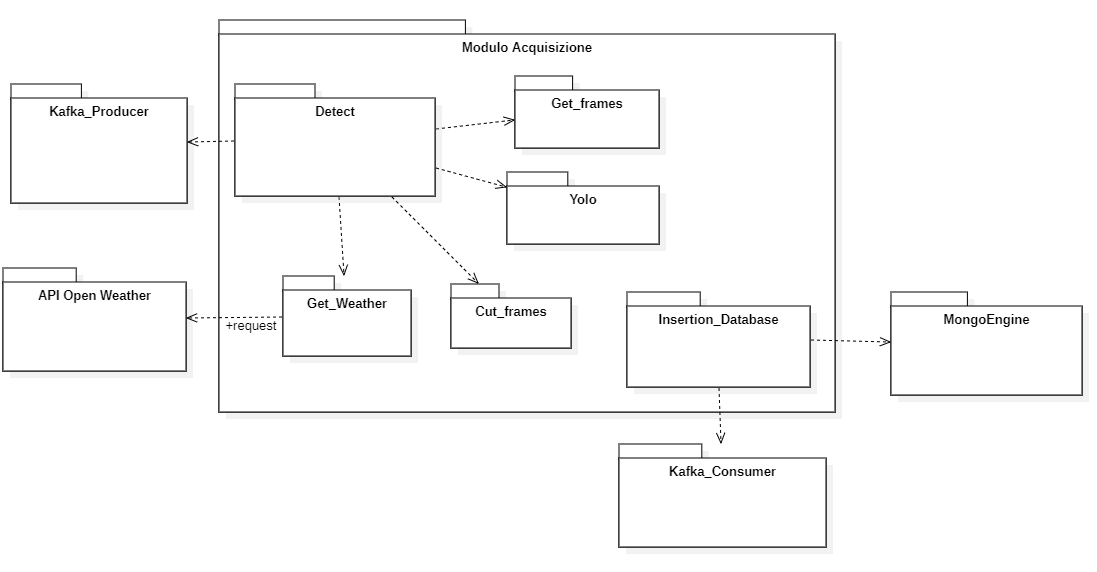
\includegraphics[scale=0.6]{../immagini/diag_PB/diag_pack_acqui.png}
    \caption{Diagramma dei package del modulo Acquisition}
  \end{center}
\end{figure}

\subsection{Diagrammi di attività}\label{ArchitetturaDelProdottoArchitetturaModuloAcquisitionDiagrammiDIAttività}
Di seguito vengono descritte le attività più importanti svolte nel modulo Acquisition.
\begin{figure}[H]
  \begin{center}
    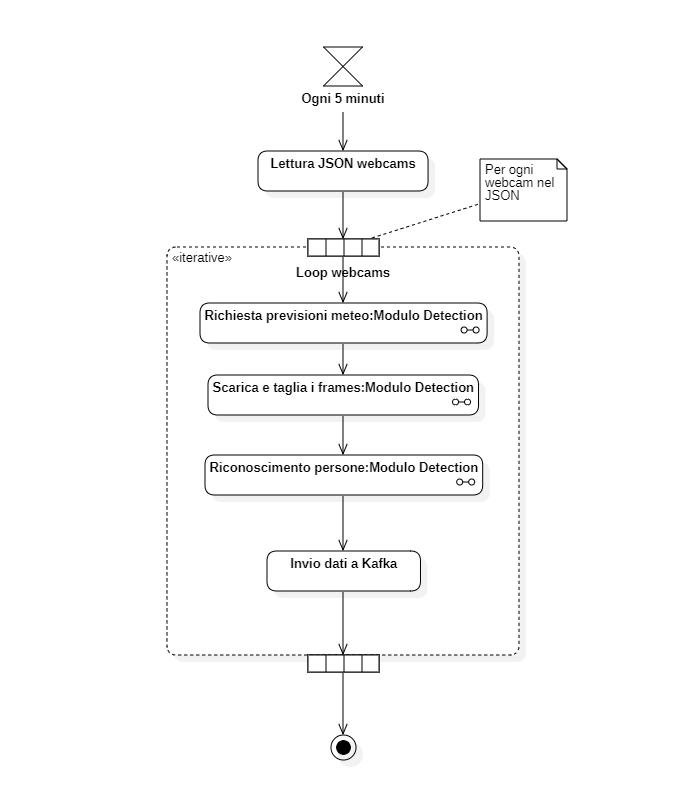
\includegraphics[scale=0.8]{../immagini/diag_PB/detection.png}
    \caption{Diagramma di attività dell'eseguibile Detection}
  \end{center}
\end{figure}


Da questo diagramma si può notare come il ciclo venga ripetuto ogni 5 minuti e per ogni webcam presente all'interno del file JSON associato.
Il lasso di tempo pari a 5 minuti è stato deciso arbitrariamente dopo aver testato la velocità di riconoscimento persone effettuato da YOLO v3.
È stato riscontrato che per elaborare 6 frame vengono impiegati circa 2 secondi per ciascuno.


\begin{figure}[H]
  \begin{center}
    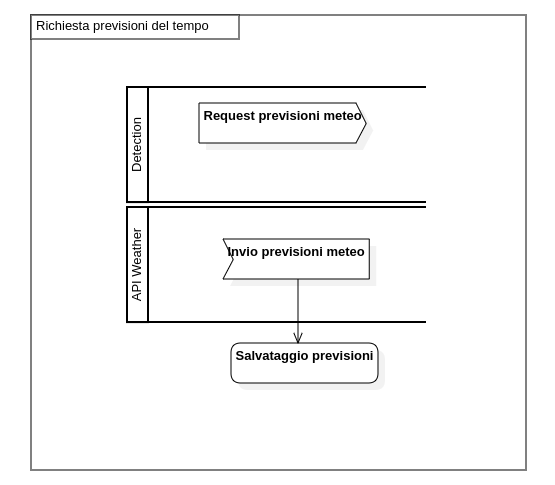
\includegraphics[scale=0.8]{../immagini/diag_PB/previsioni_del_tempo.png}
    \caption{Diagramma di sotto-attività dell'acquisizione delle previsioni meteo}
  \end{center}
\end{figure}
\begin{figure}[H]
  \begin{center}
    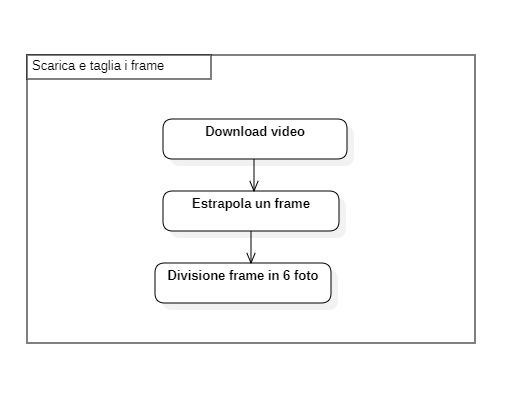
\includegraphics[scale=0.65]{../immagini/diag_PB/download_e_cut_frames.png}
    \caption{Diagramma di sotto-attività di download e taglio frame}
  \end{center}
\end{figure}
\begin{figure}[H]
  \begin{center}
    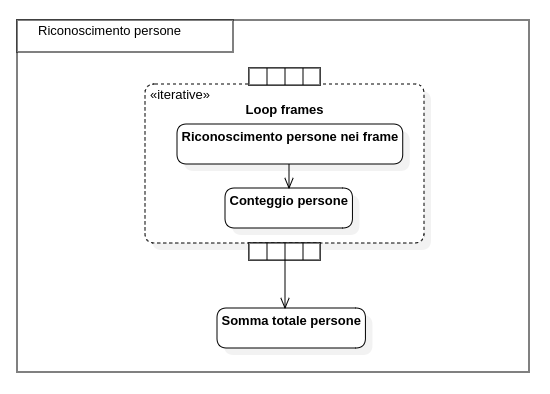
\includegraphics[scale=0.7]{../immagini/diag_PB/conta_persone.png}
    \caption{Diagramma di sotto-attività del conta persone}
  \end{center}
\end{figure}
\begin{figure}[H]
  \begin{center}
    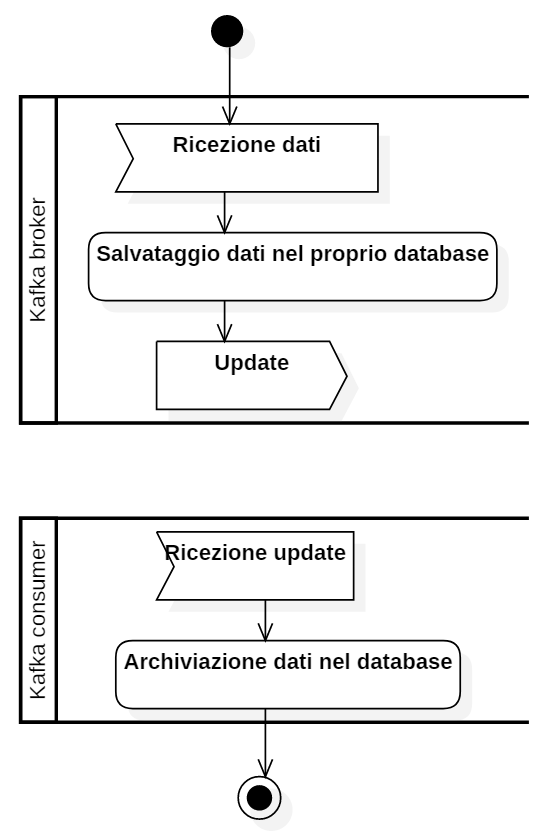
\includegraphics[scale=0.8]{../immagini/diag_PB/kafka.png}
    \caption{Diagramma di attività di Kafka}
  \end{center}
\end{figure}


\section{Architettura modulo Prediction}\label{ArchitetturaDelProdottoArchitetturaModuloPrediction}
\subsection{Diagramma dei package}\label{ArchitetturaDelProdottoArchitetturaModuloPredictionDiagrammaDeiPackage}
Nel modulo Prediction vengono utilizzate le librerie esterne Pandas$_{\scaleto{G}{3pt}}$, MongoEngine$_{\scaleto{G}{3pt}}$ e Scikit-Learn$_{\scaleto{G}{3pt}}$ (abbreviato in Sklearn nella libreria). La libreria più importante è Scikit-Learn$_{\scaleto{G}{3pt}}$ della quale utilizziamo i metodi per il Preprocessing dei dati, la creazione di modelli con Model\_selection e il tipo di modello per generare le predizioni, il Random Forest Regression.
\begin{figure}[H]
  \begin{center}
    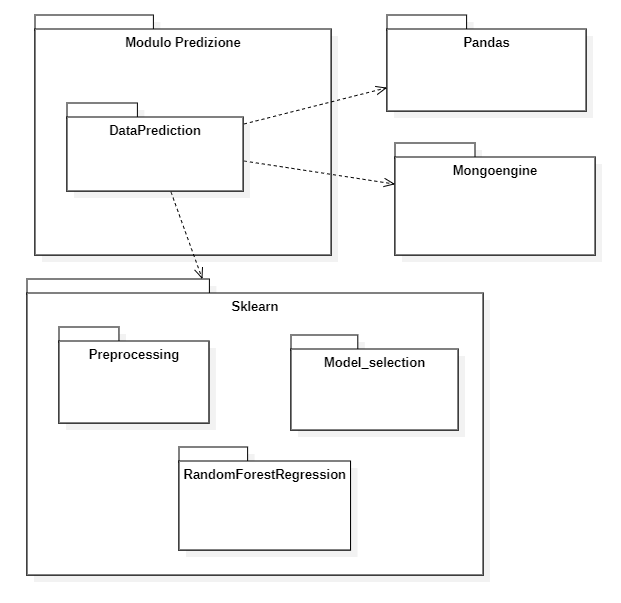
\includegraphics[scale=0.8]{../immagini/diag_PB/diag_pack_pred.png}
    \caption{Diagramma dei package del modulo Prediction}
  \end{center}
\end{figure}

\subsection{Diagramma di attività}\label{ArchitetturaDelProdottoArchitetturaModuloPredictionDiagrammaDiAttività}
Il diagramma dell'attività del modulo Prediction descrive le operazioni eseguite dal programma per generare le predizioni della zona presa in esame. Il programma legge dal file \textit{webcams.json} la lista di zone di cui bisogna effettuare le predizioni. Utilizzando le zone si prelevano i dati reali elaborati dal modulo Acquisition dal database, una volta ottenuti si controllano e vengono eliminati i dati ritenuti difettosi. Viene creato un dataset con i valori riferiti alle predizioni nel quale verranno inseriti i risultati del modello machine learning. Successivamente viene definito un modello utilizzando il tipo di regressione \textit{Random Forest Regression} e viene allenato con i valori prelevati dal database. Infine si utilizza il dataset creato precedentemente per ricavare le predizioni usando il modello allenato, a questo punto si archivia il dataset con i risultati del modello nel database.
\begin{figure}[H]
  \begin{center}
    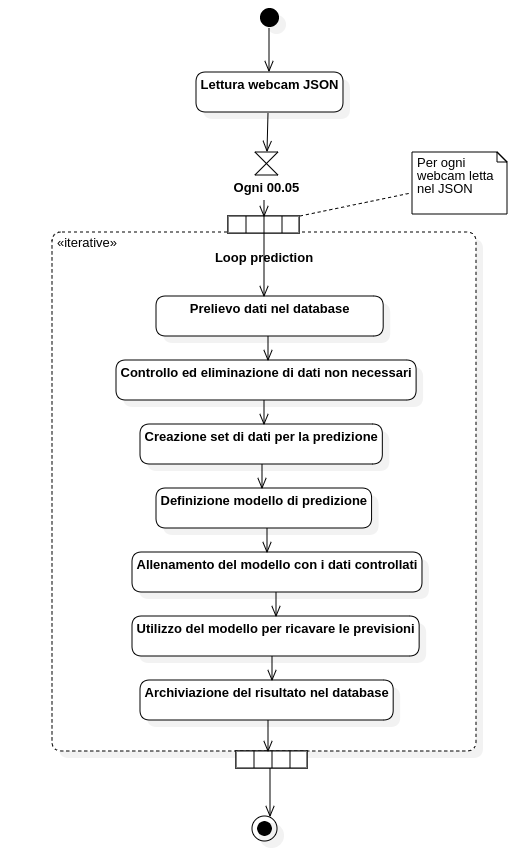
\includegraphics[scale=0.6]{../immagini/diag_PB/prediction_activity.png}
    \caption{Diagramma di attività dell'eseguibile DataPrediction}
  \end{center}
\end{figure}



\section{Architettura modulo Web-app}\label{ArchitetturaModuloWebApp}
Il modulo della web-app$_{\scaleto{G}{3pt}}$, come descritto in precedenza, è diviso in due sotto-moduli rispettivamente per il back-end$_{\scaleto{G}{3pt}}$ e front-end$_{\scaleto{G}{3pt}}$.
Il front-end è stato sviluppato seguendo le \textit{best practices} definite dalla documentazione di Vue.js e data la nostra poca conoscenza di questo linguaggio di programmmazione non è stato possibile definire un pattern strutturale per il modulo sviluppato.
L'archiviazione dei dati è stata sviluppata utilizzando un database non relazionale, il cui schema viene spiegato in seguito. Tutte le informazioni dei dati raccolti sono inserite all'interno di una collazione denominata Detection. Ogni dato è composto da 13 campi:
\begin{itemize}
	\item \textbf{\_id}: identifica univocamente il dato corrente;
	\item \textbf{id\_webcam}: individua l'id della webcam utilizzata per raccogliere il dato;
	\item \textbf{city}: individua la città in cui si trova la webcam;
	\item \textbf{location}: individua la locazione della webcam nella città;
	\item \textbf{latitude}: individua la latitudine della webcam;
	\item \textbf{longitude}: individua la longitudine della webcam;
	\item \textbf{numPeople}: individua il numero di persone presenti in quel momento;
	\item \textbf{date}: individua la data di raccolta del dato;
	\item \textbf{time}: individua l'orario di raccolta del dato;
	\item \textbf{type}: individua il tipo di dato se è 0 il dato è reale, se è 1 il dato è ricavato da una predizione;
	\item \textbf{weather\_description}: individua il tempo meteorologico;
	\item \textbf{temperature}: individua la temperatura;
	\item \textbf{day\_of\_week}: individua il giorno della settimana.
\end{itemize}
\subsection{Diagrammi dei package}\label{ArchitetturaModuloWebAppDiagrammiDeiPackage}
Di seguito vengono visualizzate le dipendenze dei due sotto-moduli, per il back-end$_{\scaleto{G}{3pt}}$ è solo necessaria la libreria del framework$_{\scaleto{G}{3pt}}$ Spring$_{\scaleto{G}{3pt}}$, mentre per il front-end$_{\scaleto{G}{3pt}}$ sono necessarie varie librerie per ogni componente della web-app$_{\scaleto{G}{3pt}}$.
\begin{figure}[H]
  \begin{center}
    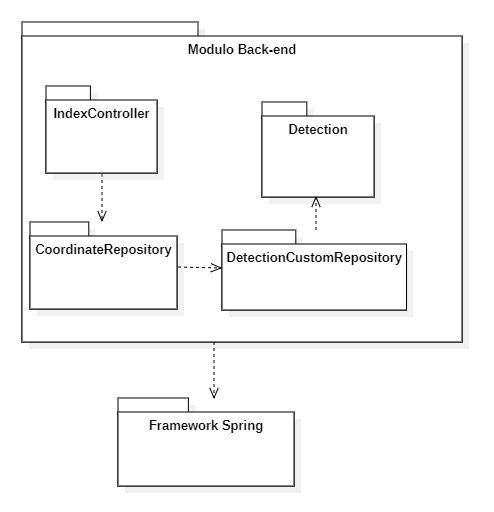
\includegraphics[scale=0.8]{../immagini/diag_PB/diag_pack_spring.png}
    \caption{Diagramma dei package di Spring}
  \end{center}
\end{figure}

\begin{figure}[H]
  \begin{center}
    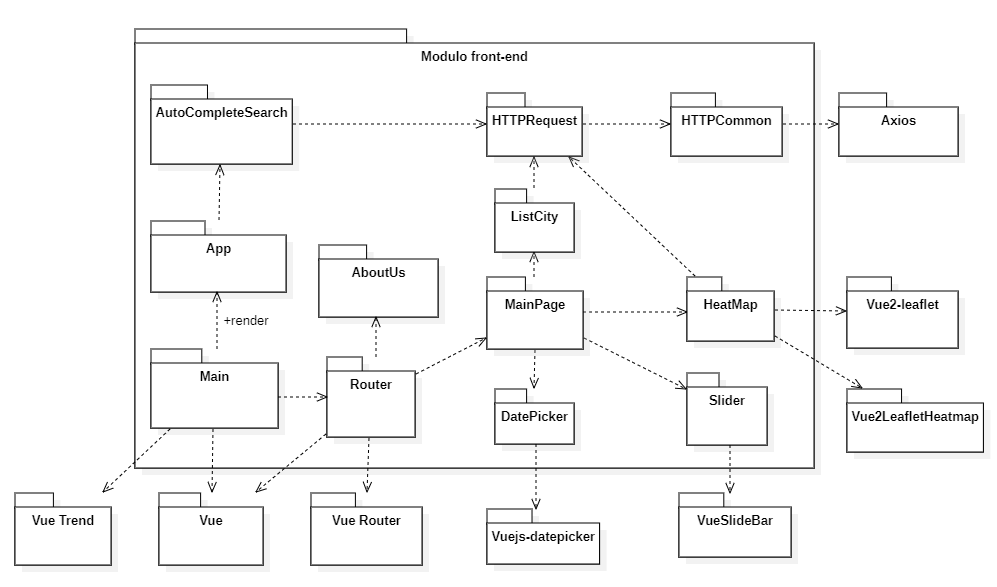
\includegraphics[scale=0.65]{../immagini/diag_PB/diag_pack_vue.png}
    \caption{Diagramma dei package del front-end in Vue}
  \end{center}
\end{figure}

\subsection{Diagrammi delle classi}\label{ArchitetturaModuloWebAppDiagrammiDelleClassi}
\begin{figure}[H]
  \begin{center}
    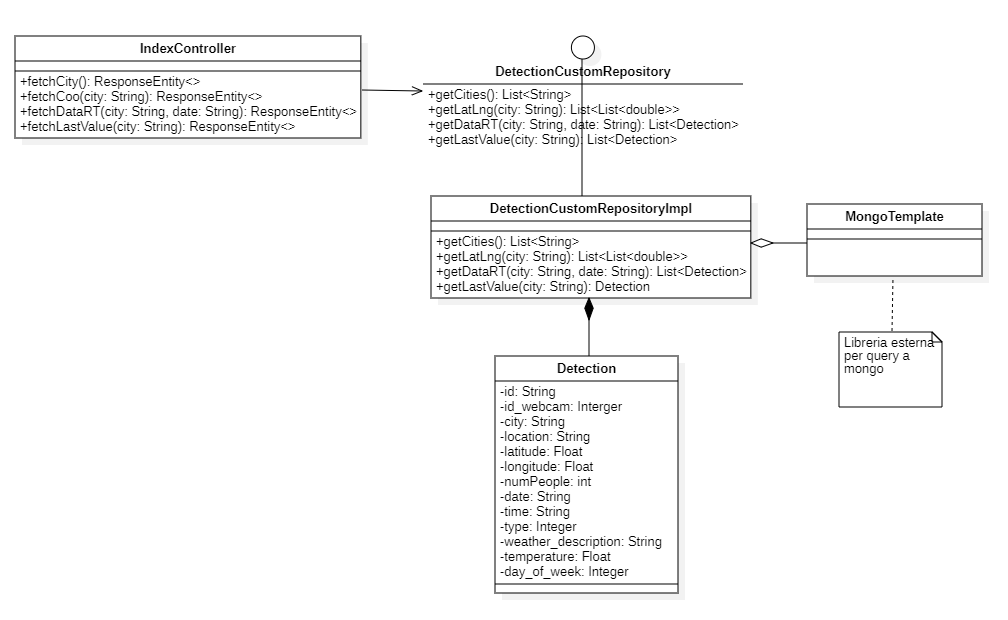
\includegraphics[scale=0.6]{../immagini/diag_PB/diag_class_spring.png}
    \caption{Diagramma delle classi di Spring}
  \end{center}
\end{figure}

\subsection{Diagramma di sequenza}\label{ArchitetturaModuloWebAppDiagrammaDiSequenza}
\begin{figure}[H]
  \begin{center}
    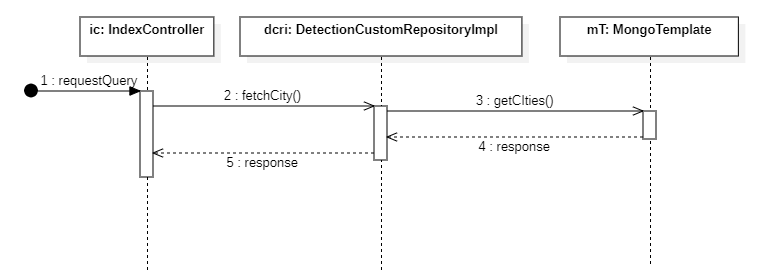
\includegraphics[scale=0.8]{../immagini/diag_PB/diag_seq_spring.png}
    \caption{Diagramma di sequenza di Spring}
  \end{center}
\end{figure}

\subsection{Diagramma di attività}\label{ArchitetturaModuloWebAppDiagrammaDiAttività}
\begin{figure}[H]
  \begin{center}
    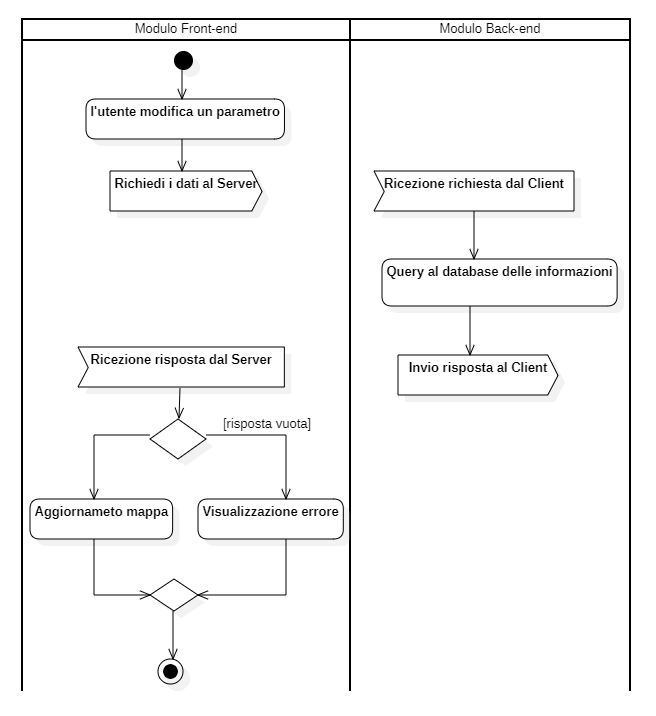
\includegraphics[scale=0.8]{../immagini/diag_PB/diag_act_front_back.png}
    \caption{Diagramma di attività del modulo Web-app}
  \end{center}
\end{figure}

	\chapter{Test}\label{Test}
Vengono di seguito elencati gli strumenti per effettuare i test che il gruppo ha sviluppato sul prodotto.

\section{Test modulo Acquisition}\label{TestModuloAcquisition}
Per il modulo di acquisizione dati sono presenti degli Unit Test all'interno della cartella \\ \texttt{acquisition/main/test}, che verificano il corretto funzionamento di alcuni metodi contenuti dagli eseguibili \texttt{detect.py} e \texttt{weather\_forecast.py}.
Si può verificare la correttezza dei metodi eseguendo i programmi all'interno della cartella, ad esempio:
\begin{lstlisting}
  python3 test_detect.py
\end{lstlisting}

\section{Test Back-end Webapp}\label{TestBackendWebapp}
Per testare il back-end$_{\scaleto{G}{3pt}}$ dell'applicazione web sono presenti alcuni test di unità; si consiglia di utilizzare un IDE con la possibilità di eseguire test in Java direttamente dall'interfaccia grafica.
Nel caso si preferisse utilizzare il terminale, è sufficiente posizionarsi all'interno della cartella \texttt{webapp/webapp/} ed eseguire il comando:
\begin{lstlisting}
  mvn clean install
\end{lstlisting}
che eseguirà tutti i test necessari.
Tali test vengono comunque eseguiti all'avvio del back-end$_{\scaleto{G}{3pt}}$ dell'applicativo.

\section{Test Front-end Webapp}\label{TestFrontendWebapp}
Per testare il frontend dell'applicazione basta posizionarsi all'interno della cartella \\ \texttt{webapp/vue-js-client-crud/} e lanciare il comando:
\begin{lstlisting}
  npm run test:unit
\end{lstlisting}
che eseguirà tutti i test riguardanti il front-end$_{\scaleto{G}{3pt}}$ con Vue.

	\chapter{Informazione aggiuntive}\label{InformazioniAggiuntive}

\section{Aggiunta di una webcam}\label{InformazioniAggiuntiveAggiuntaDiUnaWebcam}
L'aggiunta di una nuova webcam al \textit{modulo di acquisizione} è possibile attraverso dei pochi semplici passi:
\begin{enumerate}
	\item Trovare una webcam disponibile all'interno del sito \url{https://www.whatsupcams.com/};
	\item Inserire il link all'interno del file \textit{webcams.json}, presente nella cartella \textit{acquisition} seguendo lo schema prestabilito per impostare i parametri della webcam;
	\item Salvare il file per ultimare l'aggiunta.
\end{enumerate}
Per una questione di codifica, il link della webcam dev'essere conforme a quelle già presenti, ovvero provenire da \url{https://www.whatsupcams.com/}.

\section{Tracciamento degli errori}\label{InformazioniAggiuntiveTracciamentoDegliErrori}
Per tracciare gli errori è stato creato il file \textit{test.log}, presente nel percorso \textit{/acquisition/main/test/}, che tiene traccia delle eventuali eccezioni che si verificano all'interno del file \textit{detect.py}.
In \textit{test.log} vengono rappresentati dei messaggi quali:
\begin{itemize}
  \item \textit{Debug}: rappresenta la richiesta effettuata all'\textit{API Weather Forecast} per prelevare le informazioni meteo;
  \item \textit{INFO}: rappresenta il verificarsi di un'eccezione specificando data e ora di quest'ultima;
  \item \textit{Error}: specifica il tipo di errore e in quale locazione si è verificato.
\end{itemize}

	\chapter{Glossario} \label{Glossario}
\textbf{A}\\
\\
\textbf{Application client-server} \\
Indica un'applicazione basata su un'architettura di rete nella quale, generalmente, un computer si collega ad un server$_G$ per le fruizione di und eterminato servizio.\\
\\
\textbf{Applicazioni single-page} \\
S'intende una web-app$_G$ o un sito internet che può essere usato, o consultato, tramite una singola pagina, fornendo così un'esperienza più fluida e intuitiva all'utente.\\
\\
\textbf{B} \\
\\
\textbf{Back-end} \\
Interfaccia con la quale il gestore di un sito web dinamico ne gestisce i contenuti e le funzionalità. A differenza del frontend$_G$, l'accesso al backend è riservato agli amministratori del sito che possono accedere dopo essersi autenticati.\\
\\
\textbf{Build automation} \\
In informatica è l'atto di scrivere o automatizzare un'ampia varietà di compiti che gli sviluppatori software$_G$ fanno nelle loro attività quotidiane di sviluppo.\\
\\
\textbf{C} \\
\\
\textbf{Client} \\
In ambito informatico si intendo i dispositivi collegati ad un server ed in grado di scambiarvici informazioni.\\
\\
\textbf{D} \\
\\
\textbf{Database} \\
Insieme strutturati, ovvero omogenei per contenuti e formato, rappresentanti, digitalmente, un archivio dati.\\
\\
\textbf{Document-object manager} \\
Abbreviato in "DOM", in italiano è tradotto letteralmente modello a oggetti del documento, è una forma di rappresentazione dei documenti strutturati come modello orientato agli oggetti.\\
\\
\textbf{F} \\
\\
\textbf{Framework}\\
Utilizzato per descrivere la struttura operativa nella quale viene elaborato un dato software$_{\scaleto{G}{3pt}}$.
Un framework$_{\scaleto{G}{3pt}}$, in generale, include software di supporto, librerie, un linguaggio per gli script$_G$ e altri software$_{\scaleto{G}{3pt}}$ che possono aiutare a mettere insieme le varie componenti di un progetto.\\
\\
\textbf{Front-End/Front end/Frontend} \\
Parte di un sistema software che gestisce l'interazione con l'utente o con sistemi esterni che producono dati di ingresso.
Tali dati sono poi utilizzabili dal Back-end$_G$.\\
\\
\textbf{G}\\
\\
\textbf{Git}\\
Sistema di controllo gratuito a versione distribuita progettato per tenere traccia del lavoro svolto durante l'intero periodo di sviluppo del software.
Utilizzato anche per tenere traccia di tutte le modifiche fatte nei file.
I suoi punti di forza sono l'integrità dei dati e il supporto per flussi di lavoro distribuiti e non lineari.\\
\\
\textbf{GitHub}\\
GitHub$_G$ è un servizio di hosting per progetti software. Il nome deriva dal fatto che esso è una implementazione dello strumento di controllo versione distribuito Git$_G$.\\
\\
\textbf{H}\\
\\
\textbf{Heat-map}\\
Rappresentazione grafica dei dati dove i singoli valori contenuti in una matrice sono rappresentati da colori.\\
\\
\textbf{L}\\
\\
\textbf{Layout}\\
In informatica si intende la disposizione degli elementi che costituiscono una pagina internet.\\
\\
\textbf{Linux}\\
Si tratta di una famiglia di sistemi operativi open-source$_G$ pubblicati poi in varie distribuzioni.\\
\\
\textbf{M}\\
\\
\textbf{Machine-learnig}\\
Metodo di analisi dati che automatizza la costruzione di modelli analitici. È una branca dell'Intelligenza Artificiale e si basa sull'idea che i sistemi possono imparare dai dati, identificare modelli autonomamente e prendere decisioni con un intervento umano ridotto al minimo.\\
\\
\textbf{MVC}\\
È un pattern architetturale, l'acronimo MVC$_G$ sta per \textit{Model-View-Controller}.
Il \textit{model} si occupa della rappresentazione dei dati in oggetti.
Il \textit{view} gestisce la rappresentazione grafica di essi.
Infine il \textit{controller} si occupa delle interazioni degli utenti.\\
\\
\textbf{N}\\
\\
\textbf{NoSQL}\\
 È un movimento che promuove sistemi software dove la persistenza dei dati è in generale caratterizzata dal fatto di non utilizzare il modello relazionale, di solito usato dalle basi di dati tradizionali.\\
\\
\textbf{NPM}\\
Gestore di pacchetti per il linguaggio di programmazione JavaScript$_{\scaleto{G}{3pt}}$, consiste in un client$_{\scaleto{G}{3pt}}$ da linea di comando, chiamato anch'esso npm, e un database$_{\scaleto{G}{3pt}}$ online di pacchetti pubblici e privati, chiamato npm registry.\\
\\
\textbf{O}\\
\\
\textbf{Open source}\\
Un software open-source$_{\scaleto{G}{3pt}}$ è reso tale per mezzo di una licenza attraverso cui i detentori dei diritti favoriscono la modifica, lo studio, l'utilizzo e la redistribuzione del codice sorgente.\\
\\
\textbf{P}\\
\\
\textbf{Pom}\\
Acronimo di Project Object Model è l'unità fondamentale di lavoro di Maven al cui interno sono presenti le configurazioni e le informazioni riferite al progetto.\\
\\
\textbf{R}\\
\\
\textbf{Real-time}\\
Tradotto in italiano: in tempo reale.\\
\\
\textbf{Repository-Repo}\\
Ambiente di un sistema informativo in cui vengono conservati e gestiti file, documenti e metadati relativi ad un’attività di progetto.\\
\\
\textbf{Run-time system}\\
Termine utilizzato per indicare un software che fornisce i servizi necessari all'esecuzione di un programma.\\
\\
\textbf{S}\\
\\
\textbf{Script}\\
File contenente codice eseguibile.\\
\\
\textbf{Server}\\
È un componente, o sotto sistema, adibito all'elaborazione e gestione del traffico dati fornito da servizi verso altre componenti.\\
\\
\textbf{Software}\\
È l'insieme delle procedure e delle istruzioni in un sistema di elaborazione dati.\\
\\
\textbf{Spring}\\
In informatica Spring è un framework$_{\scaleto{G}{3pt}}$ open-source$_{\scaleto{G}{3pt}}$ per lo sviluppo di applicazioni su piattaforma Java$_{\scaleto{G}{3pt}}$.\\
\\
\textbf{Streaming}\\
Identifica un flusso di dati audio/video trasmessi da una sorgente a una o più destinazioni tramite una rete telematica. Questi dati vengono riprodotti man mano che arrivano a destinazione.\\
\\
\textbf{T}\\
\\
\textbf{Tomcat}\\
(Apache) è un server web open-source$_{\scaleto{G}{3pt}}$.\\
\\
\textbf{Topic}\\
Nell'ambito di Apache Kafka, si intende una categoria per utilizzata per raggruppare i messaggi.\\
\\
\textbf{U}\\
\\
\textbf{Ubuntu}\\
Sistema operativo basato su Linux$_G$, più precisamente su Debian.\\
\\
\textbf{W}\\
\\
\textbf{Web API}\\
Un'API Web è un'interfaccia di programmazione dell'applicazione per un server Web o un browser Web.
In questo caso è un sito sul quale si appoggia il software$_G$ per acquisire delle informazioni.\\
\\
\textbf{Web-app/Applicazioni web}\\
In ambito informatico si intende un'applicazione web, ovvero applicazioni fruibili mediante via web, come un sito internet che offre determinati servizi al client$_{\scaleto{G}{3pt}}$.\\
\\
\textbf{X}\\
\\
\textbf{XML}\\
È un formato di file appertenente a script$_{\scaleto{G}{3pt}}$ scritti linguaggio col medesimo nome.
Si tratta di un linguaggio di markup ossia basato su un meccanismo sintattico che consente di definire e controllare il significato degli elementi contenuti in un documento o in un testo.\\
\\


	%  glossary would go here

\end{document}
